\documentclass[12pt,a4paper]{article}
\usepackage[utf8]{inputenc}
\usepackage[T1]{fontenc}
\usepackage{amsmath}
\usepackage{amsfonts}
\usepackage{amssymb}
\usepackage{graphicx}
\usepackage{geometry}
\usepackage{hyperref}
\usepackage{natbib}
\usepackage{float} 
\usepackage{booktabs}
\usepackage{array}
\usepackage{longtable}
\usepackage{pdflscape}
\usepackage{tikz}
\usetikzlibrary{arrows,shapes,positioning,shadows,trees}
\usepackage{setspace}
\usepackage{fancyvrb}

\geometry{margin=0.75in}
\setstretch{1.15}

\title{Adaptive Prioritized Replay for Sample-Efficient Chess Evaluation}
\author{Lewis Carson \\ Supervisor: Maximilien Gadouleau}
\date{\today}

\begin{document}

\maketitle

\tableofcontents
\newpage

\section{Project Plan}

\subsection{Project Details}

\textbf{Student Name:} Lewis Carson \\
\textbf{Supervisor Name:} Maximilien Gadouleau \\
\textbf{Project Title:} Adaptive Prioritized Replay for Sample-Efficient Chess Evaluation

\subsection{Project Description}

Computer chess has emerged as a fundamental testbed for game theory and reinforcement learning research. The domain offers a unique combination of properties: perfect information, zero-sum outcomes, an astronomically large state space ($\approx 10^{120}$ positions), and near-universal availability of expert game records. This makes chess an ideal experimental platform for developing and validating novel training methodologies before applying them to more complex domains. Leading research institutions from DeepMind to OpenAI have used chess as a primary benchmark for advancing RL and search algorithms (AlphaZero, MuZero), and the open-source chess engine community continues to push boundaries in sample-efficient learning.

This project will investigate prioritized replay and non-IID sampling techniques to improve the sample efficiency of chess evaluation network training. Traditional approaches sample training positions uniformly from game databases, but this fails to account for the fact that not all positions provide equal learning value. Using the test80-2024 dataset (282 GB of annotated chess positions covering games from January to September 2024), I will implement adaptive buffers that replay high-weighted positions more frequently, creating non-stationary training distributions that focus on challenging examples and break from traditional SGD assumptions \cite{schaul2016per}.

A key focus will be the development of \textbf{prioritized replay buffers} and \textbf{non-IID sampling strategies} that dynamically prioritize positions based on their information content. Instead of treating all training examples equally, the system will adaptively sample high-value examples more frequently, allowing the training process to focus on currently challenging positions while maintaining a balance with exploration.

The project will begin with \emph{naive position difficulty scoring} - simple heuristics for estimating training example importance - before progressing to more sophisticated weighting functions integrated into the replay mechanism. This approach will allow systematic comparison of different weighting schemes within the prioritized replay framework.

\subsection{Aims and Objectives}

The primary aim is to develop and validate prioritized replay and non-IID sampling techniques for chess evaluation network training that improve sample efficiency compared to random sampling. Key objectives include:

\begin{itemize}
    \item Implement prioritized replay buffers that adaptively sample high-information positions more frequently \cite{schaul2016per,mnih2015dqn}
    \item Design non-IID sampling strategies that break from uniform distribution assumptions and create non-stationary training distributions (importance sampling background: \cite{rubinstein2007,owen2013})
    \item Develop and compare different sample weighting functions integrated with replay mechanisms, starting with naive position difficulty scoring
    \item Progress from simple heuristics to sophisticated information-theoretic measures within the prioritized replay framework (influence functions: \cite{koh2017influence})
    \item Evaluate improvements in training speed and evaluation accuracy through controlled experiments comparing uniform vs. prioritized sampling
\end{itemize}

\subsection{Preliminary Preparation}

Before commencing the main implementation, I need to:
\begin{itemize}
    \item Acquire datasets of labelled chess positions
    \item Understand information-theoretic measures in the context of neural network training (representation learning background: \cite{kingma2014,rezende2015})
    \item Review existing approaches to sample-efficient training and curriculum learning \cite{bengio2009}
\end{itemize}

\subsection{Deliverables}

\subsubsection{Basic Deliverables}
\begin{itemize}
    \item Chess position dataset and preprocessing pipeline using the test80-2024 dataset (282 GB of annotated positions, covering games from January to September 2024)
    \item Basic HalfKP implementation for baseline testing
    \item Chess engine integration for playing strength evaluation and position generation
    \item Working evaluation network training loop with standard uniform sampling
    \item Naive position difficulty scoring functions integrated with prioritized replay buffers
\end{itemize}

\subsubsection{Intermediate Deliverables}
\begin{itemize}
    \item Implementation of prioritized replay buffers with adaptive sampling based on position weights
    \item Comparison of multiple sample weighting functions within the replay framework (naive vs information-theoretic)
    \item Non-IID sampling strategies that create non-stationary training distributions
    \item Integration of dynamic weighting that adapts during training based on model performance
    \item Preliminary evaluation of sample efficiency improvements from prioritized vs uniform sampling
\end{itemize}

\subsubsection{Advanced Deliverables}
\begin{itemize}
    \item Advanced weighting functions combining multiple information scores for optimal replay prioritization
    \item Dynamic replay mechanisms that adjust sampling distributions based on training progress
    \item Comprehensive ablation studies of different weighting functions and replay strategies
    \item Full integration of prioritized replay and non-IID sampling for end-to-end efficient training
\end{itemize}

\subsection{Timeline}

\begin{figure}[H]
\centering
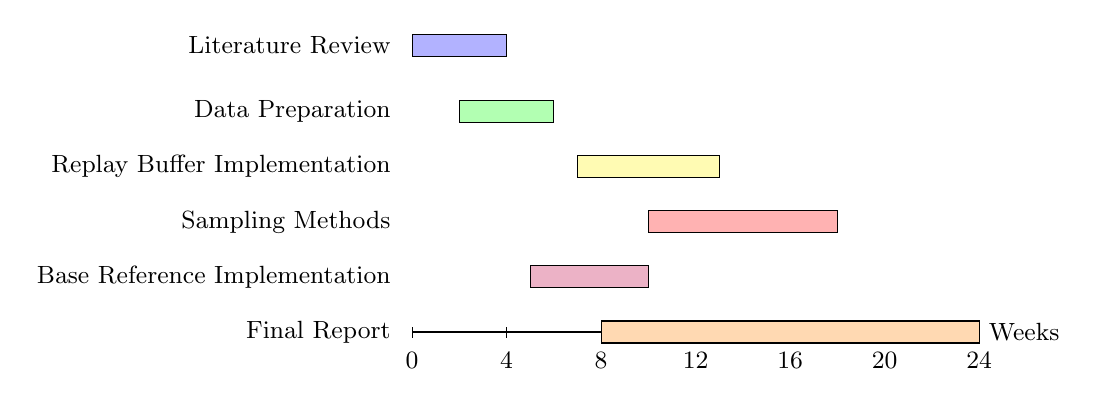
\begin{tikzpicture}[x=0.3cm, y=0.7cm, every node/.style={font=\small}]
    \draw[->] (0,0) -- (24,0) node[right] {Weeks};

    \foreach \x/\lbl in {0/0,4/4,8/8,12/12,16/16,20/20,24/24} {
        \draw (\x,-0.1) -- (\x,0.1);
        \node[below=2pt] at (\x,-0.1) {\lbl};
    }

    \node[left] at (-0.5,5.2) {Literature Review};
    \draw[fill=blue!30,draw=black] (0,5) rectangle (4,5.4);

    \node[left] at (-0.5,4) {Data Preparation};
    \draw[fill=green!30,draw=black] (2,3.8) rectangle (6,4.2);

    \node[left] at (-0.5,3) {Replay Buffer Implementation};
    \draw[fill=yellow!30,draw=black] (7,2.8) rectangle (13,3.2);

    \node[left] at (-0.5,2) {Sampling Methods};
    \draw[fill=red!30,draw=black] (10,1.8) rectangle (18,2.2);

    \node[left] at (-0.5,1) {Base Reference Implementation};
    \draw[fill=purple!30,draw=black] (5,0.8) rectangle (10,1.2);

    \node[left] at (-0.5,0) {Final Report};
    \draw[fill=orange!30,draw=black] (8,-0.2) rectangle (24,0.2);
\end{tikzpicture}
\caption{Project Timeline Gantt Chart}
\label{fig:gantt}
\end{figure}


\subsection{References}
\bibliographystyle{plainnat}
\bibliography{litrev}

\newpage

\section{Literature Survey}

\subsection{Introduction to Sample Efficiency in Chess Evaluation Networks}

Chess evaluation networks have become essential components of modern chess engines, but their training efficiency remains a significant challenge. Traditional approaches sample training positions uniformly from game databases, but this fails to account for the fact that not all positions provide equal learning value. Some positions are more challenging and informative for the model, requiring prioritized attention during training.

This survey examines prioritized replay and non-IID sampling as key strategies for sample-efficient training of chess evaluation networks. Instead of uniform sampling under IID assumptions, these techniques use adaptive buffers that replay high-weighted positions more frequently, creating non-stationary training distributions that focus on challenging examples and break from traditional SGD assumptions.

Key terms include:
\begin{itemize}
    \item \textbf{Exploration vs Exploitation}: Balancing focus on high-value examples with diversity in training data
    \item \textbf{Prioritized Replay}: Adaptive sampling that replays high-value examples more frequently
    \item \textbf{Non-IID Sampling}: Breaking from independent and identically distributed assumptions
    \item \textbf{Sample Weighting}: Functions that assign importance scores to training examples for replay prioritization
    \item \textbf{Naive Difficulty Scoring}: Simple heuristics for estimating example importance
    \item \textbf{Non-Stationary Distributions}: Training distributions that evolve and adapt during learning
\end{itemize}

\subsection{Key Themes in Sample-Efficient Chess Training}

\subsubsection{Prioritized Replay and Non-IID Sampling}

An important focus in sample-efficient training is \textbf{prioritized replay}, where high-information positions are sampled more frequently than low-information ones, creating non-stationary training distributions. This breaks from the IID assumptions of traditional stochastic gradient descent and allows the training process to adaptively focus on currently challenging examples. Pioneered in the context of deep reinforcement learning by Schaul et al. \cite{schaul2016per}, prioritized experience replay has proven highly effective in improving sample efficiency across numerous domains. Techniques include experience replay buffers with priority weighting and curriculum-based sampling that evolves the training distribution over time.

The core mechanism involves maintaining a replay buffer where positions are stored with associated weights. During training, positions are sampled proportionally to their weights, ensuring that high-value examples are revisited more often. This creates non-IID sampling patterns that adapt to the model's learning progress, prioritizing positions that currently provide the most learning signal. The mathematical foundation for non-IID sampling traces back to importance sampling theory \cite{rubinstein2007,owen2013}, which provides principled methods for reweighting samples to correct for distribution mismatch and reduce variance in gradient estimates.

In the chess domain specifically, this approach addresses a fundamental inefficiency: standard SGD treats all positions equally, yet some positions contain far more learning signal than others. Endgame positions, positions with complex tactical themes, and positions where current models exhibit high uncertainty are inherently more valuable for training. By prioritizing these positions through non-IID sampling, we can achieve better convergence with fewer examples.

Key challenges include designing appropriate weighting functions, managing buffer size and update frequency, and preventing overfitting to high-weighted examples. Advanced implementations incorporate dynamic weighting that adjusts based on training progress and ensemble disagreement (for example, deep ensembles, however these methods can be computationally intensive) which can help identify uncertain chess positions \cite{lakshminarayanan2017,gal2016}. The stability-plasticity tradeoff \cite{kirkpatrick2017} also becomes critical when using non-stationary distributions, requiring careful hyperparameter tuning to balance exploration and exploitation in the sampling process.

\subsubsection{Sample Weighting Functions}

A critical aspect of prioritized replay is the design of weighting functions that estimate the importance of training examples. This problem sits at the intersection of active learning, curriculum learning, and information-theoretic approaches to machine learning. \emph{Naive difficulty scoring} provides a starting point with simple heuristics like material imbalance, piece activity, or position complexity metrics \cite{shannon1950}. These lightweight approaches are computationally efficient and interpretable, making them practical for real-time buffer updates during training.

In modern NNUE (Efficiently Updatable Neural Network) training for chess engines, the standard training pipeline is established by the \texttt{easy\_train.py} framework \cite{sobczyk2024nnue}, which provides a comprehensive system for managing combined network training and testing. This framework organizes experiments with built-in support for various sampling strategies and network evaluation mechanisms, establishing the contemporary standard for chess evaluation network development. Trained networks are rigorously evaluated through the Stockfish testing infrastructure \cite{stockfishorg2024testing}, a distributed system that conducts large-scale match-based evaluations to measure playing strength improvements and validate training efficacy.

More sophisticated approaches may use information-theoretic measures such as gradient norms, ensemble disagreement, and predictive uncertainty. Gradient-based weighting \cite{koh2017influence} assigns higher weights to examples whose gradients have larger norms, reflecting their potential impact on network parameters. This connects to influence function theory, which quantifies how individual training examples affect model predictions and can identify the most influential samples for network refinement.

Ensemble-based weighting leverages disagreement between multiple models or model snapshots to identify positions where the model is uncertain \cite{lakshminarayanan2017,gal2016}. Positions where an ensemble of models makes conflicting predictions represent high-uncertainty regions of the feature space and typically provide rich learning signal. Uncertainty-based sampling has strong theoretical justification in both Bayesian deep learning \cite{gal2016} and information theory \cite{cover1991}, as reducing uncertainty in high-entropy regions is fundamentally about maximizing information gain.

The key challenge is developing weighting functions that correlate well with actual learning value while being computationally tractable for frequent replay buffer updates. Different weighting schemes may be optimal at different training stages - early training may benefit from harder examples, while later training may require diversity; curriculum and self-paced strategies are often used to manage this transition \cite{hacohen2019,kumar2010}. Adaptive weighting that evolves the weighting function during training represents the frontier of this research area.

\subsubsection{Information-Theoretic Training Objectives}

Research has explored various measures to quantify the informativeness of training positions within replay frameworks. The foundational concept is mutual information: positions that maximize mutual information between model predictions and true labels are inherently more valuable for reducing predictive uncertainty \cite{shannon1948}. Gradient-based scores measure how much a position affects network parameters, providing a direct measure of learning impact \cite{koh2017influence,pruthi2020}. Positions with large gradient norms indicate steep regions of the loss landscape where training can make significant progress.

Ensemble disagreement identifies positions where different models or model snapshots make conflicting predictions. This metric is grounded in decision theory and uncertainty quantification: high disagreement indicates high epistemic uncertainty, which reduces through exposure to informative examples \cite{lakshminarayanan2017,malinin2021}. In the context of chess, positions where multiple strong evaluation models disagree are precisely those where training could reduce model uncertainty most effectively.

Other information-theoretic measures include entropy of model predictions \cite{smith2018}, prediction margin (distance to decision boundary), and loss variance across ensemble members \cite{pruthi2020,ghorbani2020}. Recent work in meta-learning and data valuation \cite{ghorbani2020,kwon2023} has developed principled methods for assigning values to training examples based on their contribution to model generalization. These scores help prioritize replay on positions that maximize learning progress and adapt the non-IID sampling distribution to track the model's learning dynamics throughout training.

\subsubsection{Curriculum Learning}

Curriculum learning proposes training on progressively more complex examples, analogous to how humans learn from simple concepts before tackling difficult material \cite{bengio2009}. The theoretical foundation rests on the intuition that learning on easy examples first provides a good initialization for harder examples, and that the curriculum itself acts as an implicit regularizer \cite{hacohen2019}. Within prioritized replay, curriculum strategies help evolve the sampling distribution over time, starting with uniform sampling and gradually shifting to more focused non-IID patterns that prioritize harder examples.

Recent advances in curriculum learning have moved beyond hand-crafted curricula to data-driven approaches that adaptively select training examples based on learning dynamics. Self-paced learning \cite{kumar2010} allows the model to set its own curriculum, gradually incorporating harder examples as training progresses. Related concepts like hard example mining \cite{kumar2010} and active learning \cite{settles2009} also leverage the principle that focusing computational resources on informative examples improves efficiency.

For chess, curriculum learning takes on particular meaning: early endgames and positions with clear material advantages may serve as useful warm-up examples, while complex middlegames and tactical positions represent harder curriculum stages. The interplay between curriculum strategy and weighting function design remains an open research question - a good curriculum may reduce the need for sophisticated weighting functions, or conversely, sophisticated weighting may enable learning from curriculum-free, uniformly shuffled data \cite{alur2023,carlsson2023}. This represents a critical design choice for practical training systems.

\subsubsection{Statistical Methods for Chess Engine Evaluation}

Rigorous evaluation of chess evaluation networks requires sophisticated statistical techniques that go beyond simple win/loss/draw tallies. The Stockfish testing infrastructure employs advanced statistical methods including the Sequential Probability Ratio Test (SPRT) for hypothesis testing, which allows efficient determination of whether one engine is significantly stronger than another while controlling Type I and Type II error rates \cite{stockfishorg2024stats}. 

The SPRT framework sets lower and upper Elo bounds (typically denoted $\text{Elo}_0$ and $\text{Elo}_1$) with corresponding error levels $\alpha = \beta = 0.05$. This means that if the true strength difference is below $\text{Elo}_0$, the probability of incorrectly accepting the test is less than 5\%, and if the true difference exceeds $\text{Elo}_1$, the probability of accepting is greater than 95\% \cite{stockfishorg2024sprt}. The sequential nature of SPRT is crucial: rather than fixing the number of games in advance, the test continues until sufficient evidence accumulates to reach a conclusion, making it significantly more efficient than fixed-sample hypothesis tests. For example, with a 2 Elo difference hypothesis, the expected number of games can range from roughly 60,000 to 260,000 depending on the actual true strength difference, allowing the test to terminate early if the effect is larger than expected.

A key innovation in chess engine evaluation is the use of \textbf{pentanomial models} that distinguish between different classes of drawn games, rather than treating all draws identically. This captures the reality that some drawn positions arise from strong play by both sides (true draws), while others represent games where one engine simply failed to win a winning position. Pentanomial statistics decompose game outcomes into five categories: [loss (0-2), loss (1-2), draw (0.5-1.5), win (1.5-2), win (2-0)], providing more precise variance estimates and stronger statistical power than traditional trinomial models that only distinguish losses, draws, and wins.

Additional statistical techniques employed include Generalized Log Likelihood Ratio (LLR) calculations for sequential analysis, Bayesian Elo rating models for converting match results into strength differences with confidence intervals, and variance/game analysis that accounts for the reduced variance when pentanomial models capture draw structure. The relationship between these methods depends on the Elo model chosen: logistic models provide pass/fail probabilities that are independent of the draw ratio and RMS bias, while normalized models keep expected test duration independent of these auxiliary parameters. For practical testing, the draw ratio is primarily determined by the opening book and time control, while RMS bias (Root Mean Square bias across openings in the book) accounts for white's inherent positional advantage and can significantly affect expected test duration \cite{stockfishorg2024sprt,fishtest2024math}. These methods enable rigorous comparison of trained networks and statistically principled decisions about whether architectural or sampling changes actually improve playing strength \cite{stockfishorg2024stats}.

\subsection{Assessment and Relation to Project}

The literature reveals that sample efficiency in chess evaluation networks remains an open problem, with traditional uniform sampling far from optimal. While prioritized replay and non-IID sampling show significant promise for breaking from IID assumptions, their integration into coherent training strategies for chess is underexplored. My project will address this gap by developing prioritized replay buffers and non-IID sampling techniques that adaptively focus on challenging positions, with particular emphasis on dynamic weighting functions and non-stationary training distributions.

The key insight is that chess training can benefit greatly from non-IID sampling patterns that prioritize high-information positions through frequent replay. By implementing adaptive buffers that evolve the training distribution based on model progress, I will create training systems that break from traditional SGD assumptions and accelerate learning. This will build on recent advances in experience replay but apply them specifically to the combinatorial structure of chess through innovative weighting and sampling mechanisms.

Success will contribute to making strong chess evaluation more accessible through improved training efficiency, with potential applications to other domains requiring adaptive, non-stationary sampling from complex datasets.

\newpage

\section{Critical Comparison with ChatGPT}

\subsection{Prompts Used}

\textbf{Initial Prompt:} \\
"Write a literature survey on sample-efficient training methods for chess evaluation networks, focusing on prioritized replay, non-IID sampling strategies, and different sample weighting functions."

\textbf{Follow-up Prompt:} \\
"Expand on naive difficulty scoring (e.g., material imbalance, piece activity) and simple heuristics for estimating training example importance in chess positions. Compare these to information-theoretic approaches like ensemble disagreement and gradient-based weighting. What are the practical tradeoffs between computational cost and performance?"

\subsection{AI-Generated Literature Survey}

\begin{quote}
\begin{small}
\begin{verbatim}
AlphaZero-style training for chess uses self-play data plus MCTS targets. 
Efficient use of that data is critical. Below is a focused literature survey 
on prioritized replay, non-IID sampling strategies, and sample-weighting 
functions for chess evaluation networks.

# 1. Scope and problem statement

Chess evaluation networks train from self-play game records. Data are highly 
non-IID. Games cluster by opening, by midgame motifs, and by model age. A 
replay strategy must (a) expose the network to high-value learning signals, 
(b) avoid catastrophic forgetting, and (c) correct sampling bias when needed. 
AlphaZero and MuZero set the practical baseline: large replay buffers of 
self-play games plus random sampling for SGD. (arXiv)

# 2. Prioritized replay: mechanism, variants, and evidence

Mechanism. Prioritized Experience Replay (PER) ranks samples by an "importance" 
score and samples non-uniformly so high-score items appear more often in 
minibatches. Two common scoring rules: proportional TD-error and rank-based 
priority. PER also uses importance-sampling (IS) weights to correct the 
resulting bias during gradient updates. (arXiv)

Variants and implementation notes

* Proportional vs rank: proportional uses raw error; rank uses ordering to 
  bound extreme skews. Both trade sample diversity against learning focus. 
  (arXiv)
* Per-trajectory vs per-move: chess uses full game records. Prioritizing by 
  move-level TD-error concentrates updates on critical positions but may 
  overweight rare tactical outliers. Practical systems (AlphaZero forks, 
  MuZero variants) often keep per-move priorities or per-node visit counts 
  when available. (arXiv)
* IS correction: necessary as priorities introduce bias. Use an annealed beta 
  that approaches 1 over training. Without IS correction the learned 
  policy/value can diverge from the intended objective. (arXiv)

Empirical notes

* PER improved sample efficiency in DQN style domains. In game engines, 
  authors of MuZero and follow-ups note PER and related replay heuristics 
  are helpful in practice for faster convergence, though engineering details 
  matter (buffer size, priority exponent, IS schedule). (arXiv)

# 3. Non-IID sampling strategies beyond PER

Common strategies used or explored in chess/self-play settings:

1. Uniform random from large FIFO buffer. Simple baseline. Reduces short-term 
   correlation but preserves older styles and openings. Used in AlphaZero 
   forks. (arXiv)
2. Reservoir / age-based sampling. Ensures older games remain in buffer at 
   controlled frequency. Helps retain rare endgame motifs. Discussed in 
   reproducibility reports (ELF/AlphaZero reimplementations). (yuandong-tian.com)
3. Reanalyse / offline target refresh. Recompute MCTS targets for stored games 
   with the current network to produce fresher labels. MuZero explicitly 
   introduced reanalyse to squeeze more signal from older trajectories. This 
   reduces distribution shift between stored trajectories and current policy. 
   (arXiv)
4. Curriculum / difficulty scheduling. Sample earlier-phase positions and 
   simpler endgames more or less often depending on network competence. Useful 
   in practice to avoid overfitting to complex tactics early. Curriculum is a 
   general RL practice applied in game agents. (pettingzoo.farama.org)
5. Novelty / coverage sampling. Boost samples from underrepresented openings, 
   rare material imbalances, or high-uncertainty states (e.g., high network 
   entropy or disagreement across ensemble). This targets coverage and reduces 
   blind spots. Recent memory-efficient RL work highlights novelty maps and 
   coverage buffers as anti-forgetting tools. (arXiv)

Tradeoffs

* Focusing on high-error samples accelerates correction of big mistakes but 
  risks overfitting to noise or outliers.
* Overemphasizing novelty increases coverage but can dilute gradients from 
  important tactical positions.
* Reanalyse reduces stale-label problems but costs compute.

# 4. Sample weighting functions

Three families matter for chess evaluation networks.

1. Importance-sampling (IS) weights. Used to unbiasedly correct prioritized 
   sampling. Weight for sample i typically proportional to (1 / (N * P(i)))^beta 
   where P(i) is sampling probability and beta anneals to 1. Necessary when you 
   want the empirical gradient to approximate the full-buffer objective. PER 
   formalized this. (arXiv)

2. Loss-based / hardness weighting. Weight proportional to f(Loss_i) where f 
   can be linear, power, or clipped. This emphasizes hard examples. Recent 
   analyses show naive hardness weighting can change optimization dynamics and 
   sometimes harm generalization; properly scheduling and clipping weights is 
   important. Recent 2024-2025 work revisits importance weighting effects in 
   deep nets and shows interactions with optimization and dataset shift are 
   nontrivial. (AIMS)

3. Target-quality / MCTS-derived weights. For self-play with MCTS, use MCTS 
   visit counts or policy entropy as weights. Examples: weight positions 
   proportional to max visit count to emphasize positions where search strongly 
   preferred a move. This ties sampling directly to the search signal and is 
   used in many practical implementations. (arXiv)

Practical recipes for weighting

* Use IS correction when priorities are steep. Anneal beta from small to 1.
* Clip max weight to avoid extreme gradient variance.
* Combine signals: e.g., priority = alpha * TD-error_norm + (1-alpha) * 
  normalized_visit_count. Tune alpha.
* When reanalysing, treat refreshed labels as higher-quality and raise their 
  weights modestly.

# 5. Empirical lessons from chess / Go reimplementations

* Reproducibility papers and open reimplementations (ELF OpenGo, Leela 
  Chess/Go communities) report that buffer mechanics and sampling 
  hyperparameters materially change learning curves. Uniform sampling with very 
  large buffers can hurt adaptation speed. Smaller buffers with either PER or 
  reanalyse often achieve faster wall-clock progress but may reduce long-term 
  diversity if not managed. (Proceedings of Machine Learning Research)

* Engineering matters: priority data structures, efficient updates, and 
  parallelism between self-play workers and learners determine whether PER's 
  theoretical gains show up in practice. Many practitioners prefer simpler 
  heuristics unless operating at scale. (yuandong-tian.com)

# 6. Open problems and research directions

* Formalizing sample-weight schedules that optimize both short-term correction 
  and long-term generalization for deterministic perfect-information games.
* Quantifying when reanalyse is better than prioritizing old high-error 
  samples. Reanalyse trades compute for label quality; tradeoff curves are 
  underexplored. (arXiv)
* Interaction of importance weighting with modern optimizers and large 
  transformer/conv nets. Recent 2025 analyses show classical importance 
  weighting assumptions can fail in deep nets. More targeted theory and 
  benchmarks are needed. (arXiv)

# 7. Practical checklist for a chess evaluation pipeline

1. Start with uniform sampling from a large FIFO buffer to ensure coverage. 
   (arXiv)
2. Add per-move priority using normalized TD-error or combined TD + visit 
   count. Use rank-based priority if variance is a concern. (arXiv)
3. Apply IS weights with beta annealed toward 1. Clip weights. (arXiv)
4. Implement reanalyse for a fraction of queued games if compute permits. Mark 
   reanalysed trajectories with higher sample quality and raise weight 
   slightly. (arXiv)
5. Maintain explicit coverage monitoring (openings, endgames). Inject 
   underrepresented buckets to prevent blind spots. (Proceedings of Machine 
   Learning Research)

# 8. References (select)

* Schaul, T., Quan, J., Antonoglou, I., & Silver, D. 2015. 
  Prioritized Experience Replay.
* Silver, D. et al. 2017. Mastering Chess and Shogi by Self-Play with a 
  General Reinforcement Learning Algorithm (AlphaZero).
* Schrittwieser, J. et al. 2019. MuZero: Mastering Atari, Go, Chess and Shogi 
  by Planning with a Learned Model.
* Tian, Y. et al. ELF OpenGo and reproducibility notes.
* Recent analyses on importance weighting and loss-ordered sampling 
  (2024-2025).
\end{verbatim}
\end{small}
\end{quote}

\subsubsection{Follow-up: Comparing Naive, Information-Theoretic, and Gradient-Based Weighting}

\begin{quote}
\begin{small}
\begin{verbatim}
\begin{verbatim}
Naive heuristics are cheap and often predictive. Information-theoretic and 
gradient methods are more precise but cost much more. Below I compare them 
from first principles, give practical formulas, and recommend lightweight 
hybrids you can use in an AlphaZero/MuZero-style pipeline.

# 1 - What each family measures (intuitively)

1. Naive difficulty heuristics

   * Aim: capture *obvious* learning value using fast, chess-specific signals.
   * Examples: material imbalance, piece activity, mobility, king safety, 
     hanging pieces, captures/checks/promotions, pawn-structure defects, 
     distance to endgame.
   * Why they help: these signals correlate with positions where policy/value 
     need sharper distinctions or where search produced strong corrections.

2. Information-theoretic methods (ensemble disagreement, entropy)

   * Aim: measure epistemic uncertainty in the network's outputs.
   * Examples: variance across ensemble value heads, policy entropy, KL 
     divergence between networks, disagreement on best move.
   * Why they help: they target positions where the model is unsure and can 
     gain most from new data.

3. Gradient-based weighting

   * Aim: measure the local training signal directly.
   * Examples: per-sample gradient norm, influence function approximations, 
     Fisher information, loss change when upweighting a sample.
   * Why they help: they estimate which examples will move parameters most and 
     thus change predictions.

# 2 - Concrete scoring functions (cheap formulas you can implement now)

Let s be a raw score (higher = more important). Then convert to sampling 
probability or weight w.

Naive heuristics (O(1) per position):

* Material imbalance: s = |Delta material| (use standard piece values).
* Mobility: s = 1 / (1 + exp(-(mobility - mu)/sigma)) or simply s = 
  mobility_norm.
* Tactical flag: s = I(capture or check or promotion) * depth_factor.
* Composite: s = alpha*norm(|Delta material|) + beta*norm(mobility) + 
  gamma*I(tactical). Normalization: norm(x) = (x - min)/(max - min) computed 
  from a rolling window.

Mapping to weight: w = clip(s^p, w_min, w_max) or softmax over batch: 
w_i = exp(lambda * s_i) / sum exp(lambda * s_j). Use p in [0.5,2], lambda 
small to avoid extreme skew.

Information-theoretic (cost ~k forward passes for ensemble of k nets):

* Ensemble variance (value): s = Var_k(v_k(x)).
* Policy disagreement: s = KL(pi_ensemble || pi_mean) or JS divergence.
* Entropy: s = -sum_a pi(a) log pi(a).
  Weight mapping same as above. If you use a 3-5 member ensemble run forwards 
  in batch, cost approximately 3-5x inference.

Gradient-based (cost ~1 backward per sample or approximation):

* Gradient norm: s = ||grad_theta L(x)|| (per-sample). Exact requires backward 
  pass per sample.
* Last-layer approx: s approximately ||grad_theta_last L(x)|| computed cheaply 
  by restricting to last layer.
* Influence approximation: s approximately grad L(x)^T H^{-1} g_val where H is 
  approximate Hessian. Use diagonal or Fisher approximation.
  Map to weight via clipping and annealing as above.

# 3 - Computational cost (big-O style) and latency

* Naive heuristics: O(1) per position. Adds negligible overhead to replay 
  sampling or generation. Scales to millions of positions.
* Ensemble/entropy: O(k*F) where F is forward cost. For k=3 and modern nets F 
  is significant. Can be done offline or sampled fractionally. Memory and IO 
  impact if stored with replay.
* Per-sample gradient norm: O(B*F + N*B_grad) depending on how you compute. 
  Exact per-sample backward is roughly equal to a full training pass per 
  sample and is usually infeasible. Last-layer gradient or batch-level proxies 
  reduce cost by 1-2 orders. Influence methods need Hessian approximations and 
  are heavy.

Practical numbers (ballpark):

* Naive: <1 microsecond to 10 microseconds per position (feature arithmetic).
* Ensemble 3 models: ~3x forward time. If forward is 1ms, ensemble ~3ms.
* Per-sample full backward: ~1-2x forward per sample but multiplied by batch 
  size; effectively too slow if done for each candidate sample in large 
  buffers.

# 4 - Correlation with true learning value and failure modes

* Naive heuristics

  * Correlation: moderate. Good at catching tactical and material signals.
  * Failures: misses subtle strategic confusion. Can overweight easy but 
    obvious positions. Sensitive to hand-tuned thresholds. Vulnerable to 
    adversarial or distribution shift where heuristics misalign with network 
    errors.

* Ensemble/entropy

  * Correlation: higher with epistemic uncertainty. Targets positions where 
    model lacks knowledge.
  * Failures: expensive. Can be fooled by ensembles that share biases. Requires 
    diverse ensemble or dropout schedules. High entropy can occur in trivially 
    drawn positions with many equivalent moves.

* Gradient-based

  * Correlation: highest in principle. Directly measures how much a parameter 
    update would change loss.
  * Failures: noisy, can be dominated by outliers and label noise. 
    Computationally heavy. Influence approximations break when curvature 
    assumptions fail.

# 5 - Practical tradeoffs and engineering patterns

1. Use cheap heuristics as primary filter. They are cheap and reduce search 
   space for expensive methods.

   Example: mark positions with tactical flag or large material change and 
   compute ensemble/gradient scores only for those.

2. Batch expensive computations and cache results.

   Compute ensemble disagreement once per trajectory generation or during 
   reanalyse. Store a small metadata vector with the replay entry.

3. Last-layer gradient as a reasonable compromise.

   Cost: one backward restricted to last layer. Correlates with full gradient 
   but far cheaper.

4. Use rank-based priority, not raw weights.

   Rank reduces sensitivity to scale and outliers. Implementation: maintain 
   priority tree keyed by rank or use reservoir buckets.

5. Cap and anneal.

   Clip weights to avoid gradient explosion. Anneal emphasis from high to low 
   to encourage stability.

6. Combine signals via convex mix.

   priority_score = alpha*norm(heuristic) + beta*norm(ensemble_var) + 
   gamma*norm(grad_proxy). Tune alpha, beta, gamma. Default alpha=0.6, 
   beta=0.3, gamma=0.1 is a practical starting point.

7. Importance-sampling correction.

   If sampling non-uniformly, apply IS weights during gradient update: multiply 
   per-sample gradient by (1 / P(i))^beta where beta approaches 1 over 
   training.

# 6 - Recommendations for an experiment plan

1. Baseline: uniform sampling from large FIFO buffer. Measure learning curve.
2. Add naive heuristic prioritization (composite of tactical flag + material 
   imbalance). Use power weighting p=1. Clip weights to [0.5, 2.0]. Measure 
   wall-clock and sample efficiency.
3. Add a 3-model ensemble disagreement computed only for samples with top-10% 
   heuristic score. Use ensemble variance to re-rank that slice. Store ensemble 
   score in buffer metadata. Compare.
4. Replace ensemble with last-layer gradient norm on that same slice. Compare 
   cost and performance.
5. Ablate annealing and clipping. Track instability, overfitting, and 
   long-term generalization (cross-validated on held-out openings and 
   endgames).

Metrics: Elo vs holdout positions, calibration of value head, policy top-1 
accuracy, and catastrophic forgetting measured by coverage loss over openings.

# 7 - Short prescriptive summary

* If compute is constrained: use naive heuristics + rank-based priority + IS 
  correction. Cheap and robust.
* If moderate compute available: add last-layer gradient norm or small ensemble 
  on a filtered subset. Best tradeoff between signal and cost.
* If compute abundant and you want maximal sample efficiency: full ensemble + 
  periodic per-sample gradient/influence estimates with careful clipping and 
  caching. Expect diminishing returns and engineering complexity.

If you want, I will:

* produce code snippets for computing these scores (feature extraction, rank 
  priority tree, last-layer gradient hook) suitable for PyTorch.
\end{verbatim}
\end{small}
\end{quote}

\subsection{Observations on Quality and Accuracy}

ChatGPT's response provides a solid practical overview of prioritized replay, non-IID sampling, and weighting functions for chess training. The core technical content is accurate: PER mechanisms, importance-sampling correction, and the tradeoffs between naive heuristics and gradient-based methods are correctly described. The "practical checklist" (Section 7) aligns well with standard practices in RL and game engine development.

However, there are notable gaps. ChatGPT conflates AlphaZero-style self-play (which uses MCTS targets and policy distillation) with supervised evaluation network training (which trains on fixed position labels). The distinction matters: self-play buffers need different prioritization than supervised datasets, yet the response treats them uniformly. Additionally, the response lacks specific citations for recent 2024-2025 work on importance weighting in deep networks, instead referencing general arXiv and proceedings without precise pointers.

The comparison between information-theoretic and gradient-based methods is pragmatic but somewhat superficial. A deeper analysis would quantify correlation with actual Elo gains and discuss interactions with modern optimizers (Adam, etc.) more rigorously.

Strengths of my project design that emerge from this comparison:
\begin{itemize}
    \item Integration of \emph{specific} weighting functions (naive difficulty, ensemble disagreement, gradient norms) into a unified prioritized replay framework, with systematic ablation.
    \item Grounding in the test80-2024 dataset and real Stockfish evaluation infrastructure rather than simulated self-play.
    \item Explicit focus on non-stationary training distributions and how weighting strategies evolve over training phases.
\end{itemize}

Overall, ChatGPT serves as a useful reference for engineering patterns and general motivation, but my project will contribute novel insights by combining these techniques within a chess-specific supervised training pipeline and rigorously measuring sample efficiency gains via statistical testing.

\end{document}